% Options for packages loaded elsewhere
\PassOptionsToPackage{unicode}{hyperref}
\PassOptionsToPackage{hyphens}{url}
\PassOptionsToPackage{dvipsnames,svgnames,x11names}{xcolor}
%
\documentclass[
  10pt,
]{article}
\usepackage{amsmath,amssymb}
\usepackage{iftex}
\ifPDFTeX
  \usepackage[T1]{fontenc}
  \usepackage[utf8]{inputenc}
  \usepackage{textcomp} % provide euro and other symbols
\else % if luatex or xetex
  \usepackage{unicode-math} % this also loads fontspec
  \defaultfontfeatures{Scale=MatchLowercase}
  \defaultfontfeatures[\rmfamily]{Ligatures=TeX,Scale=1}
\fi
\usepackage{lmodern}
\ifPDFTeX\else
  % xetex/luatex font selection
  \setmainfont[]{DejaVu Serif}
  \setmonofont[]{DejaVu Sans Mono}
\fi
% Use upquote if available, for straight quotes in verbatim environments
\IfFileExists{upquote.sty}{\usepackage{upquote}}{}
\IfFileExists{microtype.sty}{% use microtype if available
  \usepackage[]{microtype}
  \UseMicrotypeSet[protrusion]{basicmath} % disable protrusion for tt fonts
}{}
\makeatletter
\@ifundefined{KOMAClassName}{% if non-KOMA class
  \IfFileExists{parskip.sty}{%
    \usepackage{parskip}
  }{% else
    \setlength{\parindent}{0pt}
    \setlength{\parskip}{6pt plus 2pt minus 1pt}}
}{% if KOMA class
  \KOMAoptions{parskip=half}}
\makeatother
\usepackage{xcolor}
\usepackage[margin=18mm]{geometry}
\usepackage{longtable,booktabs,array}
\usepackage{calc} % for calculating minipage widths
% Correct order of tables after \paragraph or \subparagraph
\usepackage{etoolbox}
\makeatletter
\patchcmd\longtable{\par}{\if@noskipsec\mbox{}\fi\par}{}{}
\makeatother
% Allow footnotes in longtable head/foot
\IfFileExists{footnotehyper.sty}{\usepackage{footnotehyper}}{\usepackage{footnote}}
\makesavenoteenv{longtable}
\usepackage{graphicx}
\makeatletter
\def\maxwidth{\ifdim\Gin@nat@width>\linewidth\linewidth\else\Gin@nat@width\fi}
\def\maxheight{\ifdim\Gin@nat@height>\textheight\textheight\else\Gin@nat@height\fi}
\makeatother
% Scale images if necessary, so that they will not overflow the page
% margins by default, and it is still possible to overwrite the defaults
% using explicit options in \includegraphics[width, height, ...]{}
\setkeys{Gin}{width=\maxwidth,height=\maxheight,keepaspectratio}
% Set default figure placement to htbp
\makeatletter
\def\fps@figure{htbp}
\makeatother
\setlength{\emergencystretch}{3em} % prevent overfull lines
\providecommand{\tightlist}{%
  \setlength{\itemsep}{0pt}\setlength{\parskip}{0pt}}
\setcounter{secnumdepth}{-\maxdimen} % remove section numbering
\ifLuaTeX
  \usepackage{selnolig}  % disable illegal ligatures
\fi
\usepackage{bookmark}
\IfFileExists{xurl.sty}{\usepackage{xurl}}{} % add URL line breaks if available
\urlstyle{same}
\hypersetup{
  colorlinks=true,
  linkcolor={Maroon},
  filecolor={Maroon},
  citecolor={Blue},
  urlcolor={Blue},
  pdfcreator={LaTeX via pandoc}}

\author{}
\date{}

\begin{document}

\section{Sparse affine substitution: complete cold software
costs}\label{sparse-affine-substitution-complete-cold-software-costs}

The sparse implementation lowers cold guest instructions in every
eligible successful comparison against both dense compression and
matched uncompressed augmentation. The frozen native summary records the
following values. Each pair solves the same original public target using
the same base, known equations and complete signed relation rows.

\begin{longtable}[]{@{}
  >{\raggedright\arraybackslash}p{(\columnwidth - 4\tabcolsep) * \real{0.3333}}
  >{\raggedright\arraybackslash}p{(\columnwidth - 4\tabcolsep) * \real{0.3333}}
  >{\raggedright\arraybackslash}p{(\columnwidth - 4\tabcolsep) * \real{0.3333}}@{}}
\toprule\noalign{}
\begin{minipage}[b]{\linewidth}\raggedright
Candidate / matched baseline
\end{minipage} & \begin{minipage}[b]{\linewidth}\raggedright
Cold Ir ratio: median {[}min, max{]}; pairs
\end{minipage} & \begin{minipage}[b]{\linewidth}\raggedright
Matrix Ir ratio: median {[}min, max{]}; pairs
\end{minipage} \\
\midrule\noalign{}
\endhead
\bottomrule\noalign{}
\endlastfoot
Ordinary: sparse / dense & 0.9128141 {[}0.8674047, 0.9288431{]}; n=10 &
0.1493742 {[}0.09986979, 0.1867933{]}; n=10 \\
Twist: sparse / dense & 0.9129475 {[}0.8636211, 0.9299975{]}; n=12 &
0.1461326 {[}0.08891192, 0.1828289{]}; n=12 \\
Ordinary: sparse / uncompressed map & 0.9955857 {[}0.9883420,
0.9969586{]}; n=10 & 0.6866483 {[}0.6444095, 0.7256114{]}; n=10 \\
Twist: sparse / uncompressed map & 0.9956286 {[}0.9887932, 0.9980363{]};
n=12 & 0.6928620 {[}0.6598903, 0.7127575{]}; n=12 \\
Ordinary: map / scalar & 0.9844571 {[}0.9811234, 0.9872640{]}; n=10 &
1.000124 {[}0.9999962, 1.000191{]}; n=10 \\
Twist: map / scalar & 0.9854769 {[}0.9812807, 0.9878889{]}; n=12 &
1.000002 {[}0.9999212, 1.000264{]}; n=12 \\
Twist full / ordinary full & 1.005008 {[}0.9735474, 1.043346{]}; n=24 &
0.9773432 {[}0.8299697, 1.178714{]}; n=24 \\
Ordinary A/A copy / original & 1.000000 {[}0.9999982, 1.000000{]}; n=24
& 1.000000 {[}1.000000, 1.000000{]}; n=24 \\
\end{longtable}

Ratios below 1 favor the candidate. These are observed case ranges, not
confidence intervals. The sparse/dense medians correspond to about 8.7\%
fewer cold instructions; sparse/uncompressed medians to about 0.4\%
fewer. This is an engineering improvement in the affine substitution
implementation, shared by ordinary and twist constructions. The
full-progression comparison has outcomes in both directions.

\subsection{Frozen experiment and
flow}\label{frozen-experiment-and-flow}

The original campaign ran once from 2026-10-30T07:21:32Z to 07:32:09Z,
with no retry or restored measurement. The November resume recovered its
final receipt; it did not rerun profiles. Source
bfcf5b74\allowbreak{}3775327a\allowbreak{}0273b2ae\allowbreak{}4d53f1d9\allowbreak{}82d29c10, freeze c65f4ed58,
worker/harness/summary pins and the exact pre-data plan are retained.
The protocol digest is
beb4cdd1\allowbreak{}3b41904c\allowbreak{}cb8f3ba1\allowbreak{}e6e17bf4\allowbreak{}d4105137\allowbreak{}bbe7cded\allowbreak{}6ec50ebe\allowbreak{}3bc3e387.

\begin{longtable}[]{@{}lr@{}}
\toprule\noalign{}
Flow & Recorded count \\
\midrule\noalign{}
\endhead
\bottomrule\noalign{}
\endlastfoot
Planned profiles & 612 \\
Attempted and completely counted computations & 612 \\
Unstarted, interrupted, resumed or excluded profiles & 0 \\
Arms crossed with each workload & 17 \\
Fresh public DLP target points & 24 \\
Q=2G control workloads & 12 \\
Existing toy curve models & 12 \\
\end{longtable}

There are two fresh target points per model, one process per
arm/workload. The same twelve models were used previously, so this is a
fresh-target confirmation on existing models. Primary ratios use only
fresh targets. All twelve Q2 positive controls recover 2; the smaller
positive arm is not a cost competitor. A/A uses the identical ordinary
implementation. Successful pairs require both source scalars verified
and all five complete problem hashes equal; missing pre-query failure
data never enters a successful ratio.

\begin{longtable}[]{@{}lr@{}}
\toprule\noalign{}
Arm / actual DLP outcome & Profiles \\
\midrule\noalign{}
\endhead
\bottomrule\noalign{}
\endlastfoot
bsgs-negation / recovered & 36 \\
bsgs / recovered & 36 \\
gp-elllog / recovered & 36 \\
ordinary-aa / recovered & 36 \\
ordinary-dense / recovered & 15 \\
ordinary-dense / underfilled & 3 \\
ordinary-dense / unsupported-alpha & 18 \\
ordinary-full / recovered & 36 \\
ordinary-map / recovered & 15 \\
ordinary-map / underfilled & 3 \\
ordinary-map / unsupported-alpha & 18 \\
ordinary-scalar / recovered & 15 \\
ordinary-scalar / underfilled & 3 \\
ordinary-scalar / unsupported-alpha & 18 \\
ordinary-sparse / recovered & 15 \\
ordinary-sparse / underfilled & 3 \\
ordinary-sparse / unsupported-alpha & 18 \\
positive / ambiguous & 24 \\
positive / recovered & 12 \\
rho-negation / recovered & 36 \\
rho / recovered & 36 \\
twist-dense / recovered & 18 \\
twist-dense / unsupported-alpha & 18 \\
twist-full / recovered & 36 \\
twist-map / recovered & 18 \\
twist-map / unsupported-alpha & 18 \\
twist-scalar / recovered & 18 \\
twist-scalar / unsupported-alpha & 18 \\
twist-sparse / recovered & 18 \\
twist-sparse / unsupported-alpha & 18 \\
\end{longtable}

\subsection{Implementation, checks and
accounting}\label{implementation-checks-and-accounting}

Dense substitution loops through every base coordinate for every
known-kernel column. Sparse substitution caches the nonzero column
supports and applies only the nonzero query coefficients. It uses
exactly the same affine parameterization, columns, constants and
elimination. Cache construction and allocation are charged to setup;
each application is charged to linear algebra. Both choices are in one
pinned worker, selected explicitly per cell. Dense/sparse equality tests
include affine offsets, arbitrary rows and zero-dimensional kernels.
This is standard sparse linear algebra. Main relation arms use generic
group decomposition; this comparison does not introduce a new algebraic
summation-polynomial solver.

The cost unit is actual single-event user-space guest instructions Ir.
The interval starts before method setup and ends after original
source-point scalar verification. Setup/discovery, queries, complete
decomposition, signs/verification/deduplication, matrix work and
recovery are exclusive phases, with resident-GP instructions included.
Input construction/parsing, loading and record serialization are
excluded equally. Each target pays its own setup. The recorded host is
x86-64 Linux, pinned CPU0/one thread, L0; clocks were used only for
resource caps.

The frozen native audit independently recomputes every raw counter and
checks 612 records. A separate strict PARI/GP process verifies 249
distinct mathematical payloads, 141 complete signed witness inventories
and six maps, including original/reduced solution fibers and source
scalars. It passed with the sole expected marker and declared stderr;
all source/runtime/binary pins remain equal. The complete rectangular
protocol/export/file-binding check passes with zero findings. The main
v17/v18 analysis-guard correction was incorporated before this new
source and protocol froze; v19 needs no post-data scientific-source
correction.

Native rho, negation/cycle-escape rho, BSGS, negation BSGS and external
PARI elllog share every target. Their per-target costs and strongest
completed measured references are retained in SUMMARY.json. The table
below reports this experiment's requested reference comparison in the
same Ir unit. The five implementations do not certify the fastest
implementation for every curve class; a same-input sparse-linear-algebra
performance comparison with FLINT/Magma is also still owed.

\begin{longtable}[]{@{}
  >{\raggedright\arraybackslash}p{(\columnwidth - 2\tabcolsep) * \real{0.5000}}
  >{\raggedright\arraybackslash}p{(\columnwidth - 2\tabcolsep) * \real{0.5000}}@{}}
\toprule\noalign{}
\begin{minipage}[b]{\linewidth}\raggedright
Arm
\end{minipage} & \begin{minipage}[b]{\linewidth}\raggedright
Cold Ir / strongest completed of five references: median {[}min, max{]};
fresh targets
\end{minipage} \\
\midrule\noalign{}
\endhead
\bottomrule\noalign{}
\endlastfoot
bsgs & 1.381343 {[}1.024072, 1.790769{]}; n=24 \\
bsgs-negation & 1.268990 {[}1.000000, 1.573439{]}; n=24 \\
gp-elllog & 1.000000 {[}1.000000, 1.027660{]}; n=24 \\
ordinary-aa & 82.47157 {[}59.89425, 119.9894{]}; n=24 \\
ordinary-dense & 90.56813 {[}66.09931, 130.5444{]}; n=10 \\
ordinary-full & 82.47157 {[}59.89428, 119.9894{]}; n=24 \\
ordinary-map & 82.73872 {[}61.59930, 114.3091{]}; n=10 \\
ordinary-scalar & 83.99382 {[}62.66246, 115.9779{]}; n=10 \\
ordinary-sparse & 81.84740 {[}61.39589, 113.6521{]}; n=10 \\
rho & 2.768657 {[}1.138028, 3.758035{]}; n=24 \\
rho-negation & 2.238160 {[}1.197390, 5.632720{]}; n=24 \\
twist-dense & 89.42789 {[}66.96837, 138.2770{]}; n=12 \\
twist-full & 81.53565 {[}61.47055, 121.4096{]}; n=24 \\
twist-map & 81.85871 {[}62.00841, 121.9607{]}; n=12 \\
twist-scalar & 82.91830 {[}63.04731, 123.4559{]}; n=12 \\
twist-sparse & 81.69797 {[}61.75862, 121.5022{]}; n=12 \\
\end{longtable}

\subsection{Evidence and next step}\label{evidence-and-next-step}

The 9,581,956-byte deterministic original raw archive has SHA-256
d78c4da4\allowbreak{}09ce88af\allowbreak{}a2f25236\allowbreak{}1988651a\allowbreak{}735e201e\allowbreak{}8947ebb2\allowbreak{}07f238fc\allowbreak{}43e22296. A
fresh download from the user-confirmed Setec store checks all 10,241
member hashes and an identical deterministic repack. Scientific
source/data remain immutable; the failed operational receipt-name
attempt and root validation records remain available. Conditional affine
Lean lemmas retain their hypotheses; native/GP replay supplies the
concrete implementation checks. Full benchmark promotion still needs
ecbench/calibrated pricing and independent-host validation.

Next, profile the remaining setup and elimination work and test
target-only recovery against full-kernel recovery, retaining the
full-span independent verifier. That proposed implementation is not part
of this result. Reuse the sparse implementation as the matched
substitution baseline in subsequent engineering tests.

\newpage

\begin{figure}
\centering
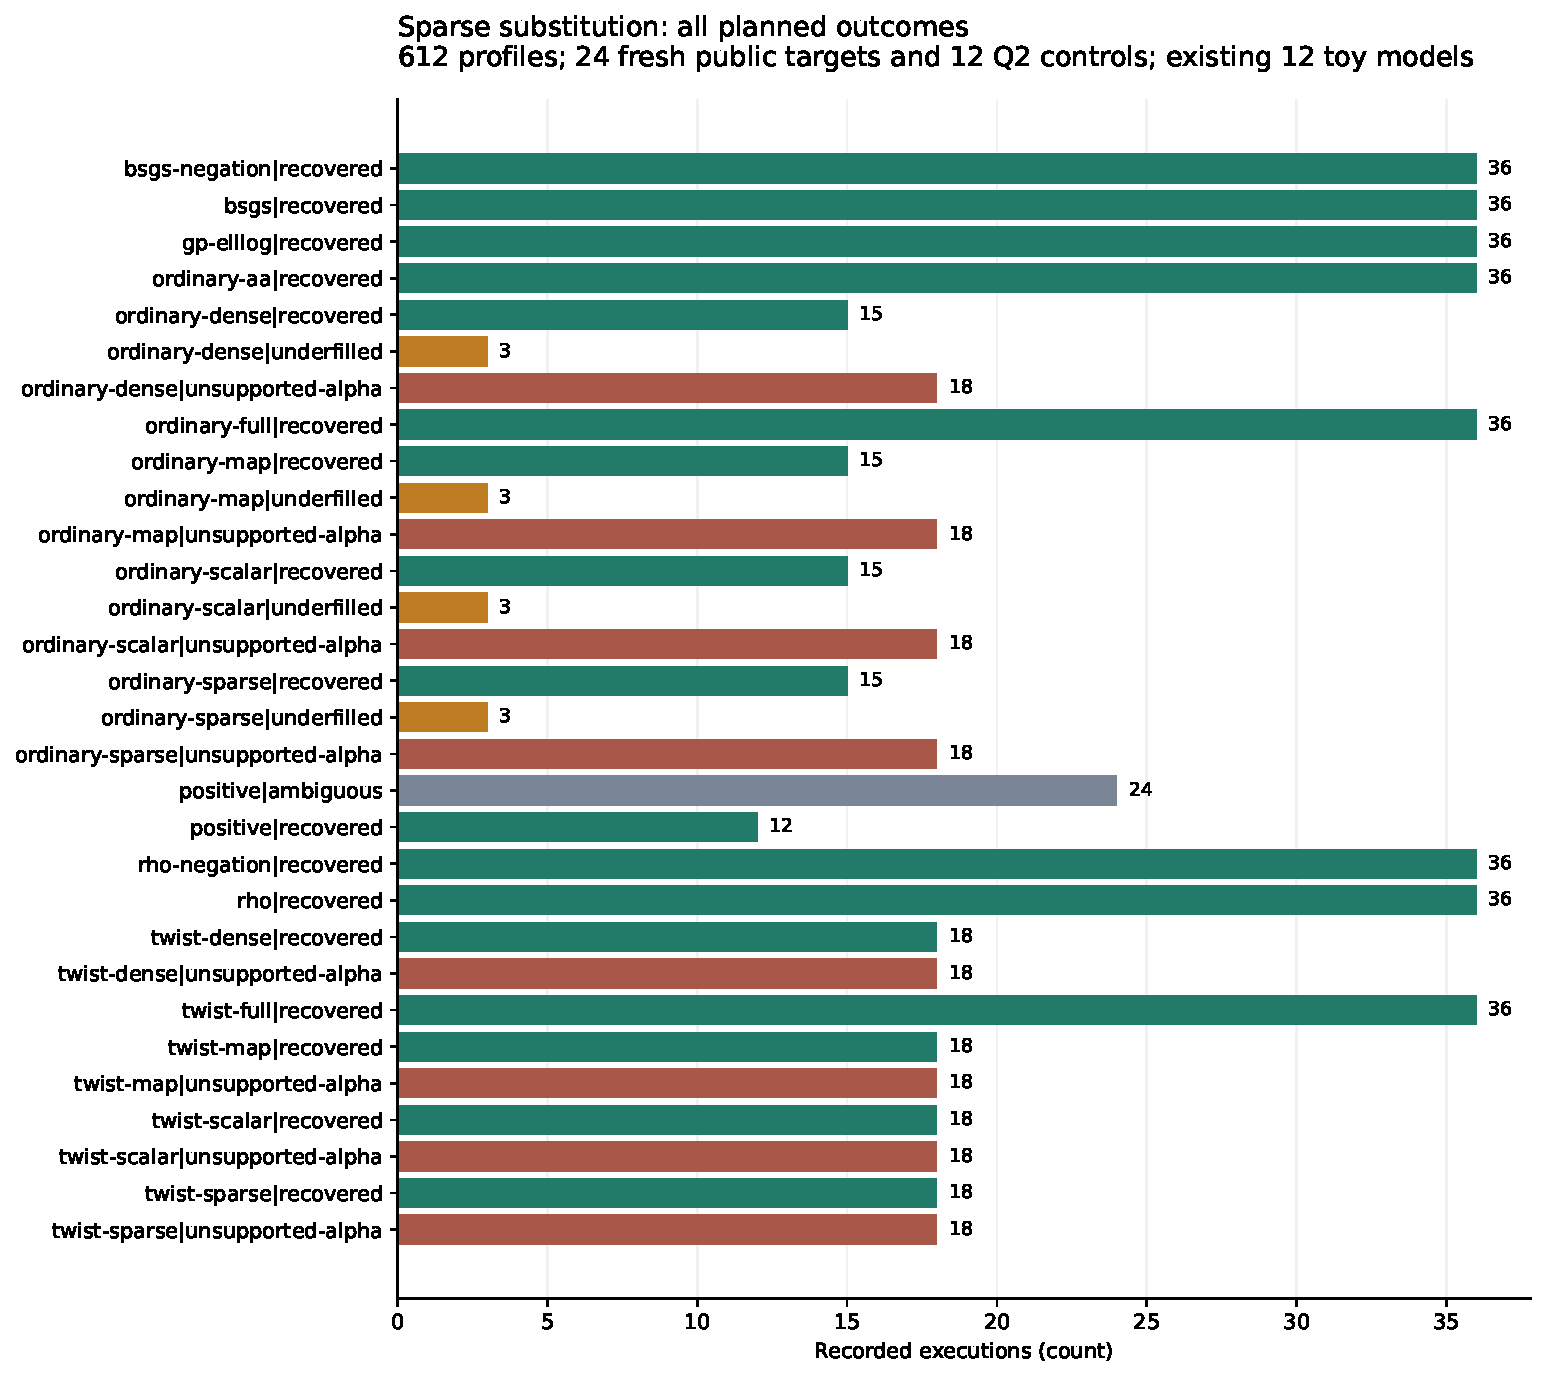
\includegraphics{OUTCOMES.pdf}
\caption{All original outcomes, including failed decompositions}
\end{figure}

\newpage

\begin{figure}
\centering
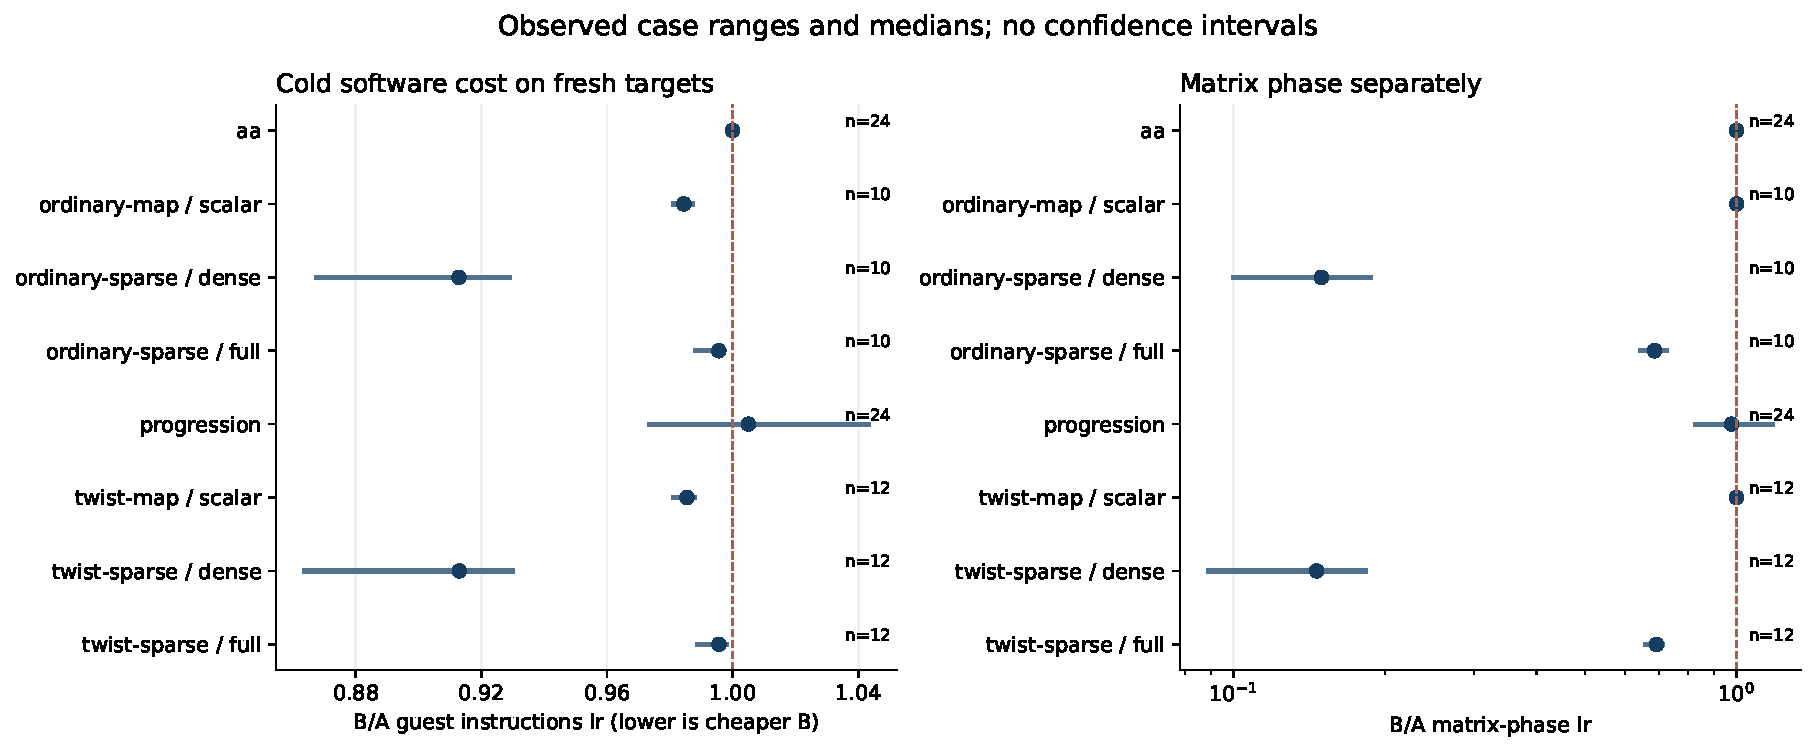
\includegraphics{RATIOS.pdf}
\caption{Frozen native ratio ranges and medians}
\end{figure}

Sources: \href{../../execution-v19/PROTOCOL.md}{protocol},
\href{../../execution-v19/FROZEN.json}{exact pins},
\href{../../execution-v19/audit-v1/ADMISSION.json}{counter and GP
admission},
\href{../../execution-v19/analysis-v1/.artifacts.json}{native summary
manifest}, \href{../../execution-v19/export-binding.stdout}{complete
export/file check}, \href{../../execution-v19/RAW_VERIFICATION.json}{raw
archive/member verification}.

\end{document}
